\section{Durchführung des Versuches}
\label{sec:Durchführung}
\subsection{Aufbau der Messapparatur}
\label{subsec:Aufbau}
Organische Szintillatoren haben gegenüber anorganischen Szintillatoren den Vorteil, dass sie eine sehr
gute Zeitauflösung besitzen. Da eine gute Zeitauflösung instrumental für die Qualität der genommenen
Daten ist, wird in diesem Versuch ein organischer Szintillator verwendet.
Dieser Szintillator befindet sich in einem Detektortank mit einem Volumen $V = \SI{50}{\liter}$.
Der Lichtpuls des Szintillators wird durch einen Photovervielfacher (im englischen Sprachraum: Photomultipliertube,
daher oft abgekürzt als PMT) in ein elektrisches Signal umgewandelt und verstärkt.
Dabei können durch thermische Effekte Elektronen emittiert werden, welche die
Messung verfälschen. Daher werden zwei PMTs verwendet, welche durch eine
Koinzidenzschaltung miteinander verbunden sind. So werden nur Signale verwendet, welche
von beiden PMTs nahezu gleichzeitig ausgesandt werden, was Fehler durch thermisches
Rauschen vermeidet.
Die Schaltung ist in Abbildung~\ref{fig:Schaltbild} dargestellt.
\begin{figure}[H]
  \centering
    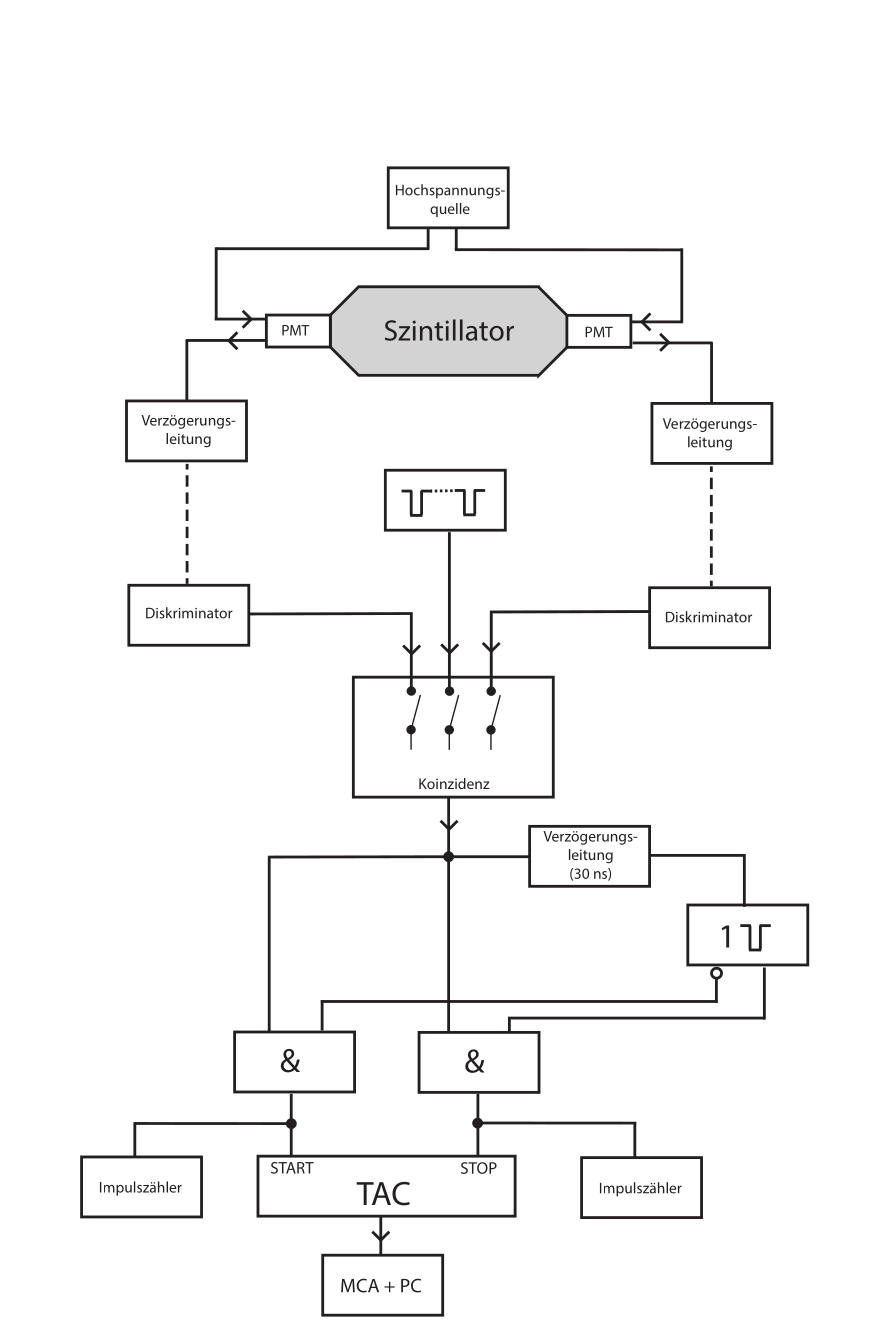
\includegraphics[width=0.7\textwidth]{pictures/Schaltbild.png}
    \caption{Schaltbild des Versuchsaufbaus. \cite{Versuchsbeschreibung}}
    \label{fig:Schaltbild}
\end{figure}
\noindent
Das Signal der PMTs wird über eine Verzögerungsleitung, welche schaltungstechnische Unterschiede
wie z.B. Kabelwege ausgleicht, durch einen Diskriminator geleitet. Dieser lässt nur Signale ab
einer gewissen Schwelle hindurch. Diese Schwelle lässt sich einstellen, wodurch Rauschen
minimiert werden kann. Das elektrische Signal, welches von dem Diskriminator ausgegeben wird,
kann auf verschiedene Breiten eingestellt werden. Hiernach folgt die bereits erwähnte Koinzidenz.
Die nun folgende Schaltung funktioniert wie eine Stoppuhr, welche das Warten auf ein Zerfallssignal
nach einer Suchzeit $T_{S}$ abbricht, was nötig wird, wenn das Myon nicht innerhalb des Detektors
zerfällt. Dies ist realisiert mittels zweier AND-Gatter, welche beide das Signal erhalten. Zusätzlich
wird das Signal auch über eine Verzögerungsleitung in einen Monoflop gesendet, welcher einen negierten
Ausgang zum linken AND-Gatter und einen normalen Ausgang zum rechten AND-Gatter besitzt. Erhält der
Monoflop das erste Signal, wird über den negierten Ausgang in das linke AND-Gatter ein Start-Signal zum
Time-to-Amplitude Converter (TAC) gesendet, wodurch die Suchzeit gestartet wird. Nach Ablauf selbiger oder
nach Erhalt eines weiteren Signals sendet der Monoflop ein Signal über den normalen Ausgang in
das rechte AND-Gatter, welches ein Stop-Signal an den TAC sendet.
Der TAC wandelt die Zeitspanne zwischen Start-Signal und Stop-Signal in eine Amplitude, dessen Höhe porportional zu der
Länge der Zeitspanne ist, um.
Der TAC ist verbunden mit einem Vielkanalanalysator (im englischen Sprachraum: Multi-Channel Analyser, daher abgekürzt als MCA).
Der MCA sortiert die erhaltenen Amplituden in ein Histogramm, welches von einem
Computer ausgelesen und gespeichert werden kann.
Zusätzlich sind an den Ausgängen der AND-Gatter Impulszähler angschlossen, sodass für eine Abschätzung
des Untergrundes auch die Myonen gezählt werden, welche nicht im Detektor zerfallen.
\subsection{Justage des Versuchsaufbaus}
\label{JustageVersuchsaufbau}
Bevor die Messung durchgeführt werden kann, muss die nach Abbildung~\ref{fig:Schaltbild} aufgebaute Schaltung justiert
werden. Die Diskriminatoren werden so eingestellt, das in etwa $30$ Impulse pro Sekunde gemessen werden.
Die Breite eines Pulses der Diskriminatoren wird einmal auf $\Delta t_\text{Puls} = \SI{15}{\nano\second}$ und einmal auf $\Delta t_\text{Puls} = \SI{10}{\nano\second}$
eingestellt, womit später auch die eigentliche Messung durchgeführt wird. Die Verzögerungsleitungen werden separat
variiert, um die Ereignisrate zu maximieren. Die Suchzeit des Monoflops wird auf $T_{S} = \SI{10}{\micro\second} $ eingestellt werden.
Unter Verwendung des Doppelimpulsgenerators wird der TAC kalibriert. Es werden verschiedene Impulsabstände eingestellt
und diese dann den einzelnen Kanälen zugeordnet. Dies wird mit $10$ Werten zwischen $\SI{0.3}{\micro\second}$
und $\SI{9.9}{\micro\second}$ durchgeführt.
